\documentclass[10pt,pdf,hyperref={unicode}]{beamer}

\mode<presentation>
{
\usetheme{boxes}
\beamertemplatenavigationsymbolsempty

\setbeamertemplate{footline}[page number]
\setbeamersize{text margin left=0.5em, text margin right=0.5em}
}

\usepackage[utf8]{inputenc}
\usepackage[english, russian]{babel}
\usepackage{bm}
\usepackage{multirow}
\usepackage{ragged2e}
\usepackage{indentfirst}
\usepackage{multicol}
\usepackage{subfig}
\usepackage{amsmath,amssymb}
\usepackage{enumerate}
\usepackage{mathtools}
\usepackage{comment}
\usepackage{multicol}
\usepackage{comment}

\usepackage[all]{xy}

\usepackage{tikz}
\usetikzlibrary{positioning,arrows}

\tikzstyle{name} = [parameters]
\definecolor{name}{rgb}{0.5,0.5,0.5}

\usepackage{caption}
\captionsetup{skip=0pt,belowskip=0pt}

\newtheorem{rustheorem}{Теорема}
\newtheorem{russtatement}{Утверждение}
\newtheorem{rusdefinition}{Определение}

% colors
\definecolor{darkgreen}{rgb}{0.0, 0.2, 0.13}
\definecolor{darkcyan}{rgb}{0.0, 0.55, 0.55}

\AtBeginEnvironment{figure}{\setcounter{subfigure}{0}}

\captionsetup[subfloat]{labelformat=empty}

%----------------------------------------------------------------------------------------------------------
\begin{comment}
\title[Пример слайдов по работе]{Пример слайдов по работе \\ курса}
\author{И.\,О.\,Фамилия}

\institute[]{Московский физико-технический институт}
\date[2022]{\small 10\;февраля\;2022\,г.}
\end{comment}
%---------------------------------------------------------------------------------------------------------
\begin{document}


%----------------------------------------------------------------------------------------------------------
\section{Multivariate Adaptive Regression Splines}
\begin{frame}{Multivariate Adaptive Regression Splines}
%~\\[-1mm]
%Заданы
%\begin{enumerate}[1)]
%	\item \ldots,
%	\item \ldots.
%\end{enumerate}
$D = \{x_i, y_i\}_{i=1}^{N}$ -- набор данных. $f(x^1, x^2, ..., x^p)$ аппроксимируем $g(x^1, x^2, ..., x^p)$. Качество аппроксимации оценивается с помощью RMSE:
$$RMSE(D) = \sqrt{\frac{1}{N}\sum_{k=1}^{N} (g(x_k) - y_k)^2}$$
%\medskip

%Параметрические семейства:
%\[
%\setlength\abovedisplayskip{0pt}
%\mathfrak{F} = \left\{\mathbf{f}| \mathbf{f} = %\text{softmax}\bigr(\mathbf{v}\bigr(\mathbf{x}\bigr)/%T\bigr), \quad \mathbf{v}: \mathbb{R}^{n} \to %\mathbb{R}^K \right\},
%\]
%\[
%\mathfrak{G} = \left\{\mathbf{g}| \mathbf{g} = %\text{softmax}\bigr(\mathbf{z}\bigr(\mathbf{x}\bigr)/%T\bigr), \quad \mathbf{z}: \mathbb{R}^n \to %\mathbb{R}^K \right\},
%\]
%где~\ldots.
$$g(x) = \sum_{m=0}^{M} a_m \cdot B_m(x), \textit{где~} B_m(x) = \prod_{k=1}^{K_m} b_{k,m}.$$
$b_{k,m}$ равен либо $max\{+(x-t),~0\}$, либо $max\{-(x-t), 0\}.$

\begin{minipage}[t]{0.2\textwidth}
\includegraphics[scale=0.25]{vis_hinge.PNG}

\end{minipage}%
\hfill
%\vrule
\hfill
\hskip-2cm
\begin{minipage}[t]{0.6\textwidth}
\vskip-2.5cm
Идея: Создать ансамбль $M(x) = \frac{1}{T}\sum_{t}^{T}a_t(x)$, где у каждой модели вход умножен на случайную ортогональную матрицу. $\overline{x} = Qx$, где $Q$ сгенерирована из распределения Хаара.
\end{minipage}


\end{frame}

%----------------------------------------------------------------------------------------------------------
\section{Результаты применения}
\begin{frame}{Результаты применения}
\justifying

На первом графике показана зависимость значения RMSE от доли признаков, использующихся в бэггинге. На втором графике изображено значение RMSE на валидационной выборке у различных алгоритмов.
\begin{figure}[h!]
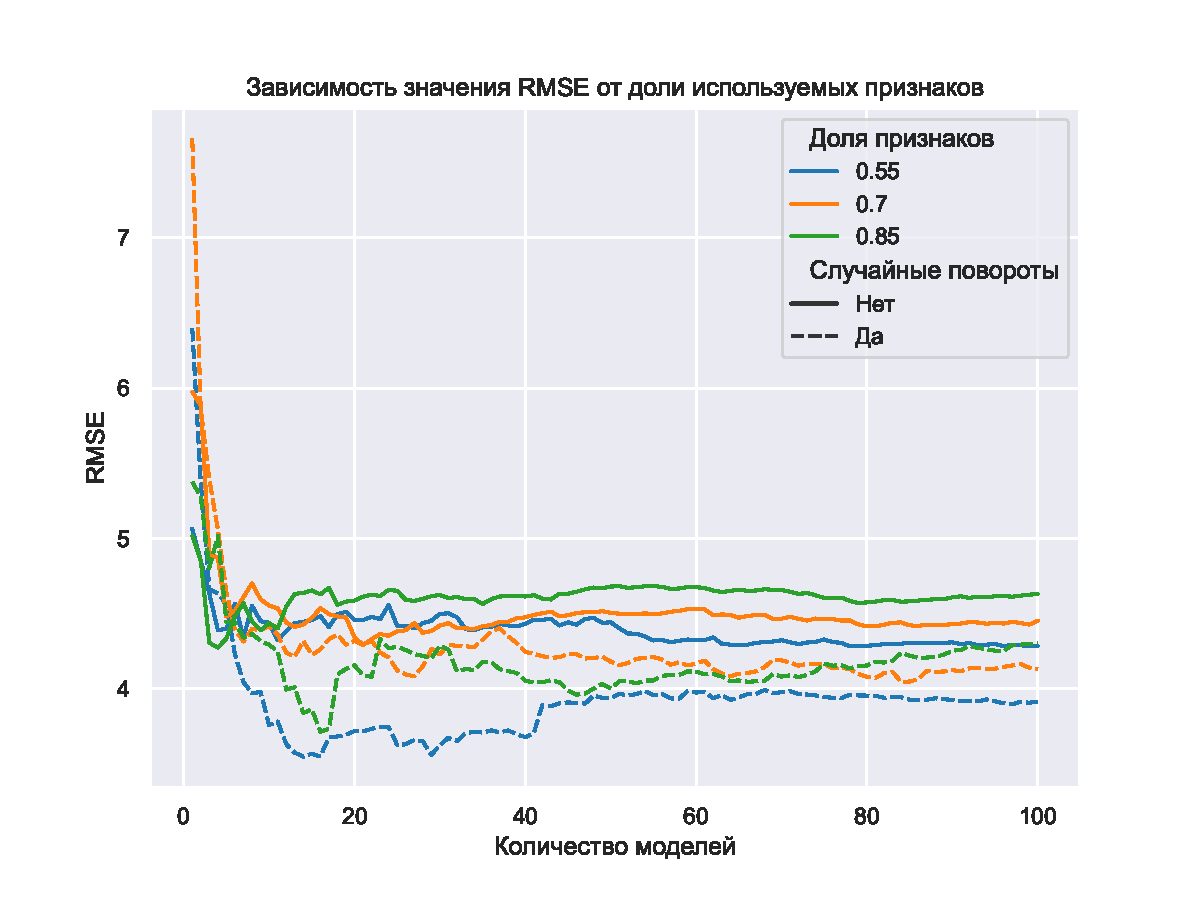
\includegraphics[width=0.48\textwidth]{../figures/be_subsample.pdf}
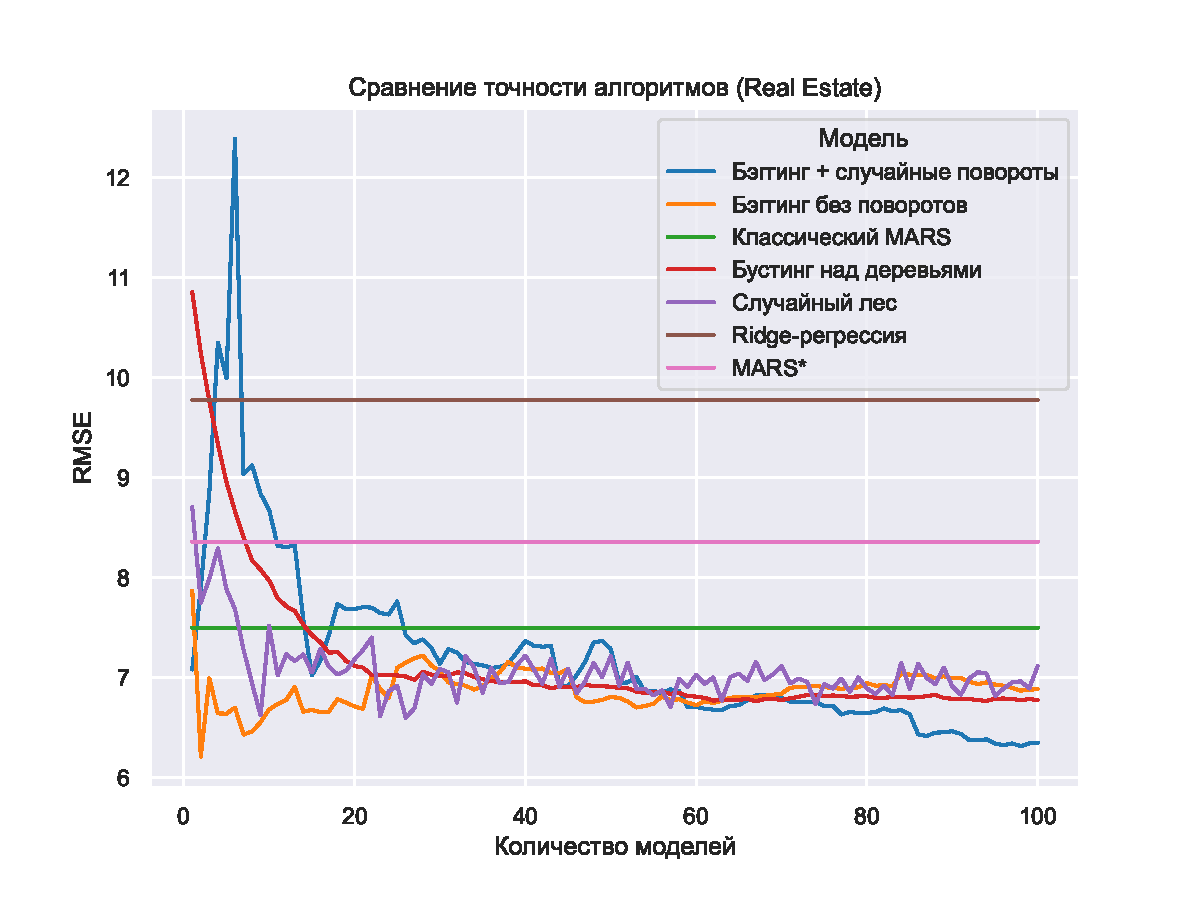
\includegraphics[width=0.48\textwidth]{../figures/re_valmodels_2.pdf}
\end{figure}

Таким образом, использование случайных поворотов позволяет добиться лучшего качества.

\end{frame}

%----------------------------------------------------------------------------------------------------------
\section{Результаты на тесте}
\begin{frame}{Выводы}

В таблице приведены результаты работы алгоритмов на тестовой выборке.
\begin{table}[h!]
\begin{center}
\begin{tabular}{|c|c|c|c|c|}
\hline
Модель\textbackslashНабор данных & BH & CH & RE & DD\\
    \hline
    Классический MARS  & 3.09 &  0.66 &  5.27 &  53.5\\
    \hline
    MARS* & 3.32 &  0.67 &  6.08 &  57.2\\
    \hline
    Бэггинг без случайных поворотов  & \textbf{2.43} & 0.63 &  4.92 &  53.1\\
    \hline
    Бэггинг + 
    случайные повороты & 2.47 & 0.62 &  \textbf{4.48} &  \textbf{52.2}\\
    \hline
    Ridge-регрессия  & 5.41 &  0.75 &  6.81 &  58.3\\
    \hline
    Случайный лес  & 2.77 & 0.63 & 5.06 &  54.1\\
    \hline
    Бустинг над 
    деревьями & 2.51 &  \textbf{0.61} &  4.85 &  54.3\\
    \hline
\end{tabular}
%\caption{\label{tab:1} Значение RMSE на тестовой выборке для каждой модели. Жирным выделен лучший результат.}
\end{center}
\end{table}
\end{frame}
%----------------------------------------------------------------------------------------------------------

\end{document} 
